\section{概要}

\index{Physics}
Physicsモジュールは物理シミュレーション機能を提供します.
\KLUDGE 主にサポートされているのは,マルチボディダイナミクスと呼ばれる剛体と関節などの拘束からなる動力学シミュレーションです.
\KLUDGE 今のところソフトボディや流体,パーティクルなどの機能はサポートされていません.

\section{Physics SDK}

\index{PHSdk}
PhysicsモジュールのすべてのオブジェクトはSDKクラス\texttt{PHSdk}によって管理されます.
\texttt{PHSdk}クラスは,プログラムの実行を通してただ1つのオブジェクトが存在するシングルトンクラスです.
\texttt{PHSdk}オブジェクトを作成するには以下のようにします.
\begin{sourcecode}
PHSdkIf* phSdk = PHSdkIf::CreateSdk();
\end{sourcecode}
\KLUDGE 通常この操作はプログラムの初期化時に一度だけ実行します.
\KLUDGE また,Frameworkモジュールを使用する場合はユーザが直接\texttt{PHSdk}を作成する必要はありません.

\texttt{PHSdk}の機能はシーンと形状の管理です.
\KLUDGE シーンに関する機能は次節で説明します.
\KLUDGE また,形状に関する機能は以下の通りです.

\begin{center}
\begin{tabular}{p{.15\hsize}p{.55\hsize}p{.2\hsize}}
\texttt{PHSdkIf} & &															\\ \midrule
\texttt{CDShapeIf*} & \texttt{CreateShape(const CDShapeDesc\&)}	& 形状を作成	\\
\texttt{CDShapeIf*}	& \texttt{GetShape(int)}					& 形状を取得	\\
\texttt{int}		& \texttt{NShape()}							& 形状の数		\\
\end{tabular}
\end{center}

\KLUDGE 異なるシーン間で形状を共有できるように,形状管理はシーンではなく\texttt{PHSdk}の機能になっています.
\KLUDGE 詳しくは\ref{chap_collision}章を参照してください.

\section{シーン}
\label{sec_physics_scene}

\index{PHScene}
\KLUDGE シーンは物理シミュレーションを行う環境を表します.
\KLUDGE 複数のシーンを作成できますが,シーン同士は互いに独立しており,ユーザが直接橋渡し処理をしない限りは影響を及ぼしあうことはありません.
\KLUDGE シーンクラスは\texttt{PHScene}で,\texttt{PHScene}オブジェクトは\texttt{PHSdk}により管理されます.

\begin{center}
\begin{tabular}{p{.15\hsize}p{.55\hsize}p{.2\hsize}}
\multicolumn{3}{l}{\texttt{PHSdkIf}}															\\ \midrule
\texttt{PHSceneIf*}	& \texttt{CreateScene(const PHSceneDesc\& desc)}			& シーンを作成		\\
\texttt{int}		& \texttt{NScene()}											& シーンの数		\\
\texttt{PHSceneIf*}	& \texttt{GetScene(int i)}									& シーンを取得		\\
\texttt{void}		& \texttt{MergeScene(PHSceneIf* scene0, PHSceneIf* scene1)}	& シーンを統合		\\
\end{tabular}
\end{center}

\KLUDGE シーンを作成するには以下のようにします.
\begin{sourcecode}
PHSceneIf* phScene = phSdk->CreateScene();
\end{sourcecode}
\KLUDGE 引数にディスクリプタを指定することもできます.
\texttt{MergeScene}は,\texttt{scene1}が保有するオブジェクトをすべて\texttt{scene0}に移動した後に\texttt{scene1}を削除します.

\KLUDGE シーンは剛体や関節などの様々な構成要素の管理を行うほか,物理シミュレーションに関する設定を行う機能を提供します.
\KLUDGE 各構成要素の作成についてはそれぞれの節で説明しますので,以下ではシミュレーション設定機能について述べます.

\begin{center}
\begin{tabular}{p{.15\hsize}p{.35\hsize}p{.4\hsize}}
\multicolumn{3}{l}{\texttt{PHSceneDesc}}										\\ \midrule
\texttt{double}		&	\texttt{timeStep}	& 時間ステップ幅					\\
\texttt{unsigned}	&	\texttt{count}		& シミュレーションしたステップ数	\\
\texttt{Vec3d}		&	\texttt{gravity}	& 重力加速度						\\
\texttt{double}		&	\texttt{airResistanceRate}	& 空気抵抗係数				\\
\texttt{int}		&	\texttt{numIteration}		& LCPの反復回数				\\
\end{tabular}
\end{center}

\begin{center}
\begin{tabular}{p{.15\hsize}p{.55\hsize}p{.2\hsize}}
\multicolumn{3}{l}{\texttt{PHSceneIf}}							  \\ \midrule
\texttt{double}		& \texttt{GetTimeStep()}					& \\
\texttt{void}		& \texttt{SetTimeStep(double)}				& \\
\texttt{unsigned}	& \texttt{GetCount()}						& \\
\texttt{void}		& \texttt{SetCount(unsigned)}				& \\
\texttt{void}		& \texttt{SetGravity(const Vec3d\&)}		& \\
\texttt{Vec3d}		& \texttt{GetGravity()}						& \\
\texttt{void}		& \texttt{SetAirResistanceRate(double)}		& \\
\texttt{double}		& \texttt{GetAirResistanceRate()}			& \\
\texttt{int}		& \texttt{GetNumIteration()}				& \\
\texttt{void}		& \texttt{SetNumIteration()}				& \\
\end{tabular}
\end{center}

\texttt{timeStep}は一度のシミュレーションステップで進める時間幅です.
\KLUDGE 小さいほどシミュレーションの精度は上がりますが,同じ時間シミュレーションを進めるのにかかる計算コストは増大します.

\texttt{count}はシーン作成後にシミュレーションした累積ステップ数です.
\texttt{count}と\texttt{timeStep}の積が経過時間を表します.

\texttt{gravity}は重力加速度ベクトルです.

\texttt{airResistanceRate}は,シミュレーションの安定性を向上するために毎ステップに各剛体の速度に掛けられる係数です.
\KLUDGE 例えば\texttt{airRegistanceRate}が$0.95$であればステップごとに速度が$95$\%になります.
\KLUDGE このように強制的に減速をかけることで,精度を犠牲に安定性を得ることができます.

\texttt{numIteration}は,拘束力を計算するために内部で実行されるアルゴリズムの反復回数です.
\KLUDGE 一般に,反復回数に関して指数関数的に拘束力の精度が向上し,計算コストは比例的に増大します.

\subsection*{シミュレーションの実行}

\KLUDGE シミュレーションを$1$ステップ進めるには\texttt{Step}関数を呼びます.

\begin{center}
\begin{tabular}{p{.15\hsize}p{.3\hsize}p{.45\hsize}}
\multicolumn{3}{l}{\texttt{PHSceneIf}}		\\ \midrule
\texttt{void}	& \texttt{Step()}	& シミュレーションを$1$ステップ進める \\
\end{tabular}
\end{center}

\texttt{Step}を実行すると,おおまかに述べて内部で次の処理が行われます.
\begin{itemize}
\item 衝突判定と接触拘束の生成
\item 拘束力の計算
\item 剛体の速度および位置の更新
\end{itemize}

\section{剛体}

\index{PHSolid}
\KLUDGE 剛体は物理シミュレーションの基本要素です.
\KLUDGE 剛体のクラスは\texttt{PHSolid}です.
\KLUDGE まず剛体を作成・管理するための\texttt{PHScene}の関数を示します.

\begin{center}
\begin{tabular}{p{.15\hsize}p{.45\hsize}p{.30\hsize}}
\multicolumn{3}{l}{\texttt{PHSceneIf}}									\\ \midrule
\texttt{PHSolidIf*}		& \texttt{CreateSolid(const PHSolidDesc\&)}	& 剛体を作成する \\
\texttt{int}			& \texttt{NSolids()}						& 剛体の数 \\
\texttt{PHSolidIf**} 	& \texttt{GetSolids()}						& 剛体配列の先頭アドレス \\
\end{tabular}
\end{center}

\KLUDGE 剛体を作成するには
\begin{sourcecode}
PHSolidIf* solid = phScene->CreateSolid();
\end{sourcecode}
\KLUDGE とします.ディスクリプタを指定して作成することもできます.
\KLUDGE また,\texttt{GetSolids}は作成した剛体を格納した内部配列の先頭アドレスを返します.
\KLUDGE したがって,例えば$0$番目の剛体を取得するには
\begin{sourcecode}
PHSolidIf* solid = phScene->GetSolids()[0];      // get 0-th solid
\end{sourcecode}
\KLUDGE とします.

\KLUDGE つぎに剛体自身の機能を説明します.

\subsection*{物性}

\begin{center}
\begin{tabular}{p{.15\hsize}p{.45\hsize}p{.30\hsize}}
\multicolumn{3}{l}{\texttt{PHSolidDesc}}							\\ \midrule
\texttt{double}		&	\texttt{mass}		& 質量					\\
\texttt{Matrix3d}	&	\texttt{inertia}	& 慣性行列				\\
\texttt{Vec3d}		&	\texttt{center}		& 質量中心				\\
\texttt{bool}		&	\texttt{dynamical}	& 物理法則にしたがうか	\\
\end{tabular}
\end{center}

\begin{center}
\begin{tabular}{p{.15\hsize}p{.45\hsize}p{.30\hsize}}
\multicolumn{3}{l}{\texttt{PHSolidIf}}								\\ \midrule
\texttt{double}		& \texttt{GetMass()}						& \\
\texttt{double} 	& \texttt{GetMassInv()}						& \\
\texttt{void} 		& \texttt{SetMass(double)}					& \\
\texttt{Vec3d} 		& \texttt{GetCenterOfMass()}				& \\
\texttt{void} 		& \texttt{SetCenterOfMass(const Vec3d\&)}	& \\
\texttt{Matrix3d} 	& \texttt{GetInertia()}						& \\
\texttt{Matrix3d} 	& \texttt{GetInertiaInv()}					& \\
\texttt{void} 		& \texttt{SetInertia(const Matrix3d\&)}		& \\
\texttt{void} 		& \texttt{CompInertia()}					& \\
\texttt{void} 		& \texttt{SetDynamical(bool)}				& \\
\texttt{bool} 		& \texttt{IsDynamical()}					& \\
\end{tabular}
\end{center}

\texttt{GetMassInv}と\texttt{GetInertiaInv}はそれぞれ質量の逆数と慣性行列の逆行列を返します.
\texttt{CompInertia}は,その剛体が持つ形状とそれらの密度をもとに剛体の質量,質量中心と慣性行列を計算し,設定します.
\texttt{dynamical}は,その剛体が物理法則に従うかどうかを指定するフラグです.
\KLUDGE もし\texttt{dynamical}が\texttt{true}の場合,その剛体に加わる力が計算され,
\KLUDGE ニュートンの運動法則にしたがって剛体の速度が変化します.
\KLUDGE 一方,\texttt{dynamical}が\texttt{false}の場合は外力による影響を受けず,設定された速度で等速運動します.
\KLUDGE これはちょうど∞の質量をもつ場合と同じです.


\subsection*{状態}

\begin{center}
\begin{tabular}{p{.15\hsize}p{.45\hsize}p{.30\hsize}}
\multicolumn{3}{l}{\texttt{PHSolidDesc}}							\\ \midrule
\texttt{Vec3d}	&	\texttt{velocity}		& 速度					\\
\texttt{Vec3d}	&	\texttt{angVelocity}	& 角速度				\\
\texttt{Posed}	&	\texttt{pose}			& 位置と向き			\\
\end{tabular}
\end{center}

\begin{center}
\begin{tabular}{p{.2\hsize}p{.5\hsize}p{.20\hsize}}
\multicolumn{3}{l}{\texttt{PHSolidIf}}									\\ \midrule
\texttt{Vec3d}			& \texttt{GetVelocity()}						& \\
\texttt{void} 			& \texttt{SetVelocity(const Vec3d\&)}			& \\
\texttt{Vec3d} 			& \texttt{GetAngularVelocity()}					& \\
\texttt{void} 			& \texttt{SetAngularVelocity(const Vec3d\&)}	& \\
\texttt{Posed} 			& \texttt{GetPose()}							& \\
\texttt{void} 			& \texttt{SetPose(const Posed\&)}				& \\
\texttt{Vec3d} 			& \texttt{GetFramePosition()}					& \\
\texttt{void} 			& \texttt{SetFramePosition(const Vec3d\&)}		& \\
\texttt{Vec3d} 			& \texttt{GetCenterPosition()}					& \\
\texttt{void} 			& \texttt{SetCenterPosition(const Vec3d\&)}		& \\
\texttt{Quaterniond} 	& \texttt{GetOrientation()}						& \\
\texttt{void} 			& \texttt{SetOrientation(const Quaterniond\&)}	& \\
\end{tabular}
\end{center}

\texttt{velocity}, \texttt{angVelocity}, \texttt{pose}はそれぞれグローバル座標系に関する剛体の速度,角速度,位置および向きを表します.
\texttt{[Get|Set]FramePosition}はグローバル座標系に関する剛体の位置を取得/設定します.
\KLUDGE これに対して\texttt{[Get|Set]CenterPosition}は剛体の質量中心の位置を取得/設定します.
\KLUDGE 偏心している剛体はローカル座標原点と質量中心が一致しないことに注意してください.
\texttt{[Get|Set]Orientation}はグローバル座標系に関する剛体の向きを取得/設定します.


\subsection*{力の印加と取得}

\KLUDGE 剛体に加わる力には
\begin{itemize}
\item ユーザが設定する外力
\item 重力
\item 関節や接触から加わる拘束力
\end{itemize}
\KLUDGE の$3$種類があり,それぞれについて並進力とトルクがあります.
\KLUDGE ここで,重力は重力加速度と剛体の質量より決まり,拘束力は拘束条件を満たすように内部で自動的に計算されます.
\KLUDGE 以下ではユーザが剛体に加える外力を設定・取得する方法を示します.

\begin{center}
\begin{tabular}{p{.2\hsize}p{.5\hsize}p{.20\hsize}}
\multicolumn{3}{l}{\texttt{PHSolidIf}}								\\ \midrule
\texttt{void} 	& \texttt{AddForce(Vec3d)}					& \\
\texttt{void} 	& \texttt{AddTorque(Vec3d)}					& \\
\texttt{void} 	& \texttt{AddForce(Vec3d, Vec3d)}			& \\
\texttt{Vec3d} 	& \texttt{GetForce()}						& \\
\texttt{Vec3d} 	& \texttt{GetTorque()}						& \\
\end{tabular}
\end{center}

\KLUDGE 並進力を加えるには\texttt{AddForce}を使います.
\begin{sourcecode}
solid->AddForce(Vec3d(0.0, -1.0, 0.0));
\end{sourcecode}
\KLUDGE とすると剛体の質量中心に並進力$(0, -1, 0)$が加わります.ただし力はグローバル座標系で表現されます.
\KLUDGE 一方
\begin{sourcecode}
solid->AddTorque(Vec3d(1.0, 0.0, 0.0));
\end{sourcecode}
\KLUDGE とすると剛体の質量中心に関してモーメント$(1, 0, 0)$が加わります.
\KLUDGE 作用点を任意に指定するには
\begin{sourcecode}
solid->AddForce(Vec3d(0.0, -1.0, 0.0), Vec3d(0.0, 0.0, 1.0));
\end{sourcecode}
\KLUDGE とします.この場合は並進力$(0, -1, 0)$が作用点$(0, 0, 1)$に加わります.
\KLUDGE ここで作用点の位置は剛体のローカル座標ではなくグローバル座標で表現されることに注意してください.
\texttt{AddForce}や\texttt{AddTorque}は複数回呼ぶと,それぞれで指定した外力の合力が最終的に剛体に加わる外力となります.

\KLUDGE 外力を取得するには\texttt{GetForce},\texttt{GetTorque}を使います.
\KLUDGE ただし,これらの関数で取得できるのは直前のシミュレーションステップで剛体に作用した外力です.
\KLUDGE したがって直前のシミュレーションステップ後に\texttt{AddForce}した力は取得できません.
\KLUDGE %シミュレーションの実行と力の印加,取得に関するフローをFig.\,\ref{fig_addforce}に示します.


\section{関節}

\begin{figure}[t]
\begin{center}
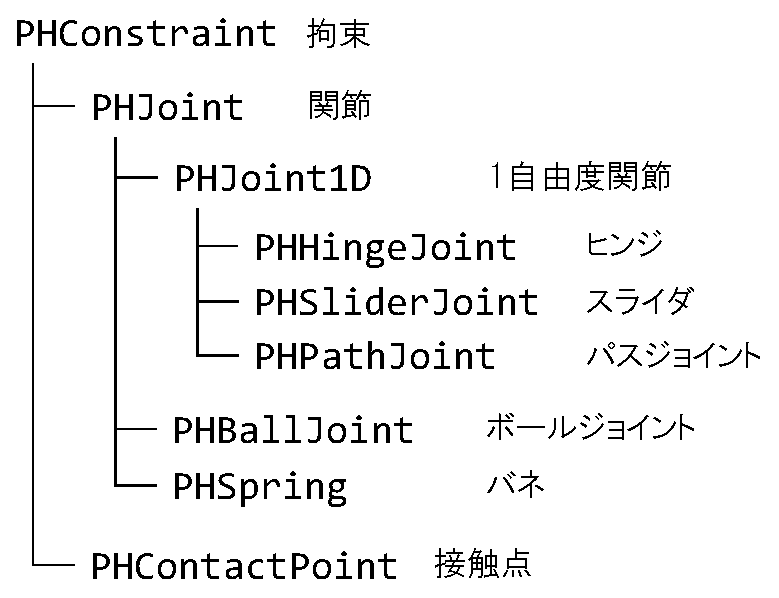
\includegraphics[width=.5\hsize]{fig/phconstraint.eps}
\end{center}
\caption{Constraint class hierarchy}
\label{fig_phconstraint}
\end{figure}

\index{PHConstraint}
\index{PHJoint}
\KLUDGE 拘束とは剛体と剛体の間に作用してその相対的運動に制約を加える要素です.
\KLUDGE 拘束のクラス階層をFig.\,\ref{fig_phconstraint}に示します.
\KLUDGE まず拘束は関節と接触に分かれます.関節はユーザが作成しますが,接触は衝突判定結果にもとづいて自動的に生成・削除されます.
\KLUDGE 関節はさらにいくつかの種類に分けられます.

\KLUDGE 細かな説明は後回しにして,まずは関節の作成方法から見ていきます.

\subsection*{関節の作成}

\KLUDGE 以下ではもっとも使用頻度の高いヒンジの作成を例にとって関節の作成方法を説明します.
\KLUDGE ヒンジを作成するには次のようにします.
\begin{sourcecode}
PHSolidIf* solid0 = phScene->GetSolids()[0];
PHSolidIf* solid1 = phScene->GetSolids()[1];

PHHingeJointDesc desc;
desc.poseSocket.Pos() = Vec3d( 1.0, 0.0, 0.0);
desc.posePlug.Pos()   = Vec3d(-1.0, 0.0, 0.0);
PHHingeJointIf* joint
    = phScene->CreateJoint(solid0, solid1, desc)->Cast();
\end{sourcecode}
\KLUDGE 作成したい関節の種類に応じたディスクリプタを作成し,これを\texttt{PHScene}の\texttt{CreateJoint}関数に渡して関節を作成します.
\KLUDGE このとき,ディスクリプタとともに連結したい剛体のインタフェースも渡します.
\texttt{CreateJoint}は\texttt{PHJointIf*}を返しますので,作成した関節のインタフェースを得るには\texttt{Cast}で動的キャストします.

\KLUDGE 関節に関する\texttt{PHScene}の関数を以下に示します.

\begin{center}
\begin{tabular}{p{.15\hsize}p{.75\hsize}p{.0\hsize}}
\multicolumn{3}{l}{\texttt{PHSceneIf}}													\\ \midrule
\texttt{PHJointIf*}	& \texttt{CreateJoint(PHSolidIf*, PHSolidIf*, const PHJointDesc\&)}	& \\
\texttt{int}		& \texttt{NJoint()}													& \\
\texttt{PHJointIf*}	& \texttt{GetJoint(int i)}											& \\
\end{tabular}
\end{center}

\texttt{NJoint}はシーン中の関節の個数を返します.\texttt{GetJoint}は\texttt{i}番目の関節を取得します.


\subsection*{ソケットとプラグ}

\index{そけっと@ソケット}
\index{ぷらぐ@プラグ}
\begin{figure}[t]
\begin{center}
\begin{tabular}{c}
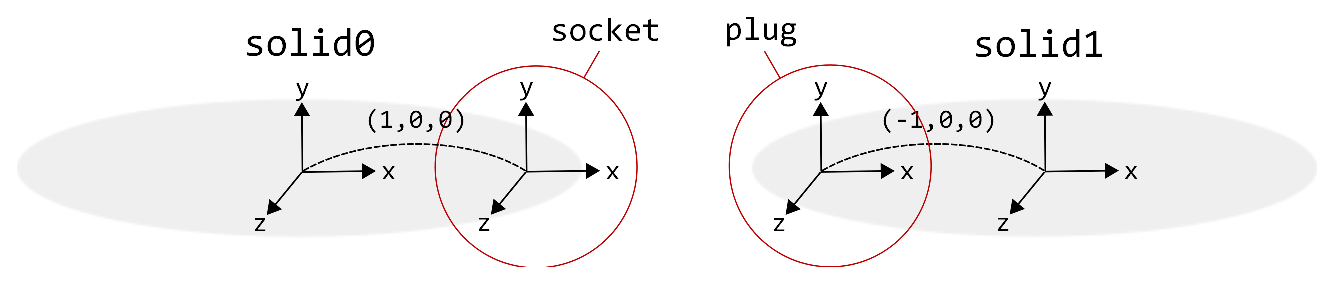
\includegraphics[clip, width=.5\hsize]{fig/socket_plug1.eps} \\
(a) before connection \\
\\
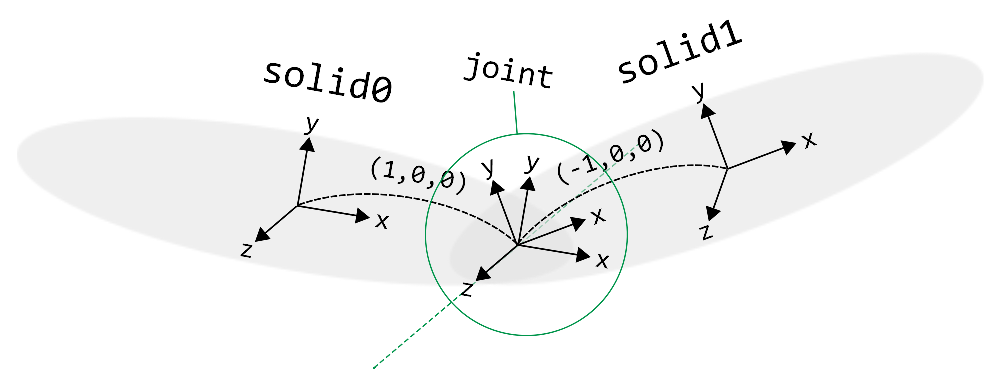
\includegraphics[clip, width=.5\hsize]{fig/socket_plug2.eps} \\
(b) after connection \\
\end{tabular}
\end{center}
\caption{Socket and plug}
\label{fig_socket_plug}
\end{figure}


\KLUDGE さて,上の例でディスクリプタに値を設定している箇所に注目してください.この部分で関節の取り付け位置を指定しています.
Springheadでは,ソケットとプラグと呼ばれるローカル座標系を用いて関節の取り付け位置を表現します.
\KLUDGE ソケットとプラグとは,その名前から連想するように,連結する剛体に取り付ける金具のようなものです.
\texttt{CreateJoint}の第$1$引数の剛体にソケットがつき,第$2$引数の剛体にプラグがつきます.
\KLUDGE ソケットとプラグがそれぞれの剛体のどの位置に取り付けられるかを指定するのがディスクリプタの\texttt{poseSocket}と\texttt{posePlug}です.
\KLUDGE 上の例ではソケットの位置が$(1,0,0)$,プラグの位置が$(-1,0,0)$でした(Fig.\,\ref{fig_socket_plug}(a)).
\KLUDGE この場合はFig.\,\ref{fig_socket_plug}(b)のように剛体が連結されます.
\KLUDGE 後述するように,ヒンジはソケットとプラグのz軸を一致させる拘束です.
\KLUDGE したがって連結された剛体同士はソケットとプラグのz軸を回転軸として相対的に回転することができます.

\KLUDGE ソケットとプラグに関するディスクリプタとインタフェースを紹介します.

\begin{center}
\begin{tabular}{p{.15\hsize}p{.35\hsize}p{.40\hsize}}
\multicolumn{3}{l}{\texttt{PHConstraintDesc}}					\\ \midrule
\texttt{Posed}	&	\texttt{poseSocket}	& ソケットの位置と向き	\\
\texttt{Posed}	&	\texttt{posePlug}	& プラグの位置と向き	\\
\end{tabular}
\end{center}

\begin{center}
\begin{tabular}{p{.15\hsize}p{.50\hsize}p{.25\hsize}}
\multicolumn{3}{l}{\texttt{PHConstraintIf}}								\\ \midrule
\texttt{PHSolidIf*}	& \texttt{GetSocketSolid()}							& ソケット側の剛体 \\
\texttt{PHSolidIf*} & \texttt{GetPlugSolid()}							& プラグ側の剛体 \\
\texttt{void} 		& \texttt{GetSocketPose(Posed\&)}					& \\
\texttt{void} 		& \texttt{SetSocketPose(const Posed\&)}				& \\
\texttt{void} 		& \texttt{GetPlugPose(Posed\&)}						& \\
\texttt{void} 		& \texttt{SetPlugPose(const Posed\&)}				& \\
\texttt{void} 		& \texttt{GetRelativePose(Posed\&)}					& 相対的な位置と向き \\
\texttt{void} 		& \texttt{GetRelativeVelocity(Vec3d\&, Vec3d\&)}	& 相対速度 \\
\texttt{void} 		& \texttt{GetConstraintForce(Vec3d\&, Vec3d\&)}		& 拘束力 \\
\end{tabular}
\end{center}
\KLUDGE %	Vec3d GetMotorf();
\KLUDGE %	Vec3d GetLimitf();

\texttt{GetRelativePose}はソケット座標系から見たプラグ座標系の相対的な位置と向きを取得します.
\KLUDGE 同様に,\texttt{GetRelativeVelocity}はソケットからみたプラグの相対速度をソケット座標系で取得します.
\KLUDGE ここで第$1$引数が並進速度,第$2$引数が角速度です.
\texttt{GetConstraintForce}はこの拘束が剛体に加えた拘束力を取得します(第$1$引数が並進力,第$2$引数がモーメント).
\KLUDGE 具体的には,ソケット側剛体に作用した拘束力をソケット座標系で表現したものが得られます.
\KLUDGE プラグ側剛体には作用反作用の法則によって逆向きの力が作用しますが,これを直接取得する関数は用意されていません.





\KLUDGE % --- --- --- --- --- --- --- --- --- --- --- --- --- --- ---
\subsection*{関節の種類}

Springheadで使用可能な関節の種類は

\begin{itemize}
\item ヒンジ (\texttt{PHHingeIf})
\item スライダ (\texttt{PHSliderIf})
\item パスジョイント (\texttt{PHPathJointIf})
\item ボールジョイント (\texttt{PHBallJointIf})
\item バネ (\texttt{PHSpringIf})
\end{itemize}

\KLUDGE の5種類です.種類ごとに,自由度・拘束の仕方・変位の求め方が異なります.


\KLUDGE % --- --- --- --- ---
\subsubsection*{ヒンジ}

\begin{fig}
\epscapopt{phhingejoint}{Hinge joint}{width=0.5\hsize}
\end{fig}

\index{PHHingeJoint}
\index{ひんじ@ヒンジ}
\KLUDGE ヒンジは$1$軸回転関節です.
\KLUDGE ヒンジは,\Fig{phhingejoint}に示すようにソケットとプラグのz軸が一致するように拘束します.
\KLUDGE このときソケットのy軸とプラグのy軸の成す角(x軸同士でも同じことですが)が関節変位となります.

\KLUDGE 関節変位を取得するAPIは$1$自由度関節(\texttt{PH1DJointIf})で共通です.そのためヒンジに限らずスライダ・パスジョイントでも使用できます.

\begin{reference}{PH1DJointIf}
\classmember{double GetPosition()}
\KLUDGE 関節の変位を取得します.変位のはかり方は関節の種類に依存します.
\end{reference}

\KLUDGE % --- --- --- --- ---
\subsubsection*{スライダ}

\begin{fig}
\epscapopt{phsliderjoint}{Slider joint}{width=0.5\hsize}
\end{fig}

\index{PHSliderJoint}
\index{すらいだ@スライダ}
\KLUDGE スライダは$1$自由度の直動関節です.
\KLUDGE スライダは,\Fig{phsliderjoint}に示すようにソケットとプラグのz軸が同一直線上に乗り,かつ両者のx軸,y軸が同じ向きを向くように拘束します.
\KLUDGE このときソケットの原点からプラグの原点までが関節変位となります.



\KLUDGE % --- --- --- --- ---
\subsubsection*{パスジョイント}

\index{PHPathJoint}
\index{ぱすじょいんと@パスジョイント}
\KLUDGE パスジョイントはソケットとプラグの相対位置関係を$1$パラメータの自由曲線で表現する関節です.詳しくは後述します.

T.B.D.



\KLUDGE % --- --- --- --- ---
\subsubsection*{ボールジョイント}

\begin{fig}
  \begin{tabular}{cc}
    \epsopt{phballjoint}{width=0.45\hsize} & \epsopt{swingtwist}{width=0.35\hsize} \\
    (a) & (b)
  \end{tabular}
  \labelcap{phballjoint}{Ball Joint}
\end{fig}

\index{PHBallJoint}
\index{ぼーるじょいんと@ボールジョイント}
\KLUDGE ボールジョイントは$3$自由度の回転関節です.
\KLUDGE ボールジョイントは\Fig{phballjoint}(a)に示すようにソケットとプラグの原点が一致するように拘束します.
\KLUDGE ソケット座標系をプラグ座標系に変換するようなクォータニオンが変位となります.

\KLUDGE 一方で,ボールジョイントの変位はオイラー角の一種であるSwing-Twist座標系(\Fig{phballjoint}(b))で取得することもできます.
\KLUDGE ソケットとプラグのz軸同士がなす角をスイング角(Swing),プラグのz軸をソケットのx-y平面への射影がソケットのx軸となす角をスイング方位角(Swing-Dir),プラグのz軸周りの回転角度をツイスト角(Twist)と呼びます.Swing-Twist座標系は,後述するボールジョイントの関節可動範囲の指定に用います.

\KLUDGE この2種類の変位は,それぞれに対応した関数で取得することができます.
\begin{reference}{PHBallJoint}
\classmember{Quaterniond GetPosition()}
\KLUDGE ソケット座標系をプラグ座標系に変換するようなクォータニオンを返します.

\classmember{Vec3d GetAngle()}
Swing-Twist座標系で表現された関節変位を返します.
\end{reference}


\subsubsection*{バネ}

\index{PHSpring}
\index{ばね@バネ}

\begin{fig}
\epscapopt{phspring}{Spring}{width=0.5\hsize}
\end{fig}

\KLUDGE 剛体間を連結するダンパ付きバネです.ソケット座標系とプラグ座標系が一致するときが自然状態で,位置の変位・姿勢の変位に比例して自然状態に戻すような力・モーメントを発生します.並進運動に作用するバネ・ダンパ係数と,回転運動に作用するバネ・ダンパ係数はディスクリプタによってそれぞれ設定できます.

\begin{lightreference}{PHSpringDesc}
\ifLwarp
  \def\member#1#2{\multicolumn{2}{l}{\texttt{#1}} & #2 \\}
\fi
\member{Vec3d spring}{並進運動に対するバネ係数}
\member{Vec3d damper}{並進運動に対するダンパ係数}
\member{double springOri}{回転運動に対するバネ係数}
\member{double damperOri}{回転運動に対するダンパ係数}
\end{lightreference}


\subsection*{有効化と無効化}

\begin{center}
\begin{tabular}{p{.15\hsize}p{.45\hsize}p{.30\hsize}}
\multicolumn{3}{l}{\texttt{PHConstraintDesc}}					\\ \midrule
\texttt{bool}	&	\texttt{bEnabled}	& 有効/無効フラグ		\\
\end{tabular}
\end{center}

\begin{center}
\begin{tabular}{p{.15\hsize}p{.50\hsize}p{.25\hsize}}
\multicolumn{3}{l}{\texttt{PHConstraintIf}}						\\ \midrule
\texttt{void}	& \texttt{Enable(bool)}					& \\
\texttt{bool} 	& \texttt{IsEnabled()}					& \\
\end{tabular}
\end{center}

\KLUDGE 有効な拘束は拘束力を生じます.無効化された拘束は存在しないのと同じ状態になりますが,
\KLUDGE 削除するのと異なりいつでも再度有効化することができます.
\KLUDGE 作成直後の拘束は有効化されています.





\subsection*{関節制御}

\subsubsection*{$1$自由度関節の場合}

\begin{center}
\begin{tabular}{p{.15\hsize}p{.45\hsize}p{.30\hsize}}
\multicolumn{3}{l}{\texttt{PHJoint1DDesc}}								\\ \midrule
\texttt{double}	&	\texttt{spring}			& 可動範囲下限				\\
\texttt{double}	&	\texttt{damper}			& 可動範囲上限				\\
\texttt{double}	&	\texttt{targetPosition}	& 可動範囲制限用バネ係数	\\
\texttt{double}	&	\texttt{targetVelocity}	& 可動範囲制限用ダンパ係数	\\
\texttt{double}	&	\texttt{offsetForce}	& \\
\texttt{double}	&	\texttt{fMax}			& \\
\end{tabular}
\end{center}

\begin{center}
\begin{longtable}{p{.15\hsize}p{.45\hsize}p{.30\hsize}}
\multicolumn{3}{l}{\texttt{PHJoint1DIf}}						\\ \midrule
\texttt{double}	& \texttt{GetPosition()}				& 関節変位を取得 \\
\texttt{double} & \texttt{GetVelocity()}				& 関節速度を取得 \\
\texttt{void} 	& \texttt{SetSpring(double)}			& \\
\texttt{double} & \texttt{GetSpring()}					& \\
\texttt{void} 	& \texttt{SetDamper(double)}			& \\
\texttt{double} & \texttt{GetDamper()}					& \\
\texttt{void} 	& \texttt{SetTargetPosition(double)}	& \\
\texttt{double} & \texttt{GetTargetPosition()}			& \\
\texttt{void} 	& \texttt{SetTargetVelocity(double)}	& \\
\texttt{double} & \texttt{GetTargetVelocity()}			& \\
\texttt{void} 	& \texttt{SetOffsetForce(double)}		& \\
\texttt{double} & \texttt{GetOffsetForce()}				& \\
\texttt{void} 	& \texttt{SetTorqueMax(double)}			& 最大関節トルクを設定 \\
\texttt{double} & \texttt{GetTorqueMax()}				& 最大関節トルクを取得 \\
\end{longtable}
\end{center}

\KLUDGE 関節を駆動する力$f$は次式で与えられます.
\begin{align*}
f = K(p_0 - p) + D(v_0 - v) + f_0
\end{align*}
\KLUDGE ここで$p$,$v$はそれぞれ関節変位と関節速度で\texttt{GetPosition},\texttt{GetVelocity}で取得できます.
\KLUDGE その他の記号とディスクリプタ変数との対応は以下の通りです.
\begin{center}
\begin{tabular}{ll}
$K$		&	\texttt{spring}				\\
$D$		&	\texttt{damper}				\\
$p_0$	&	\texttt{targetPosition}		\\
$v_0$	&	\texttt{targetVelocity}		\\
$f_0$	&	\texttt{offsetForce}
\end{tabular}
\end{center}
\KLUDGE 上の式はバネ・ダンパモデルとPD制御則の二通りの解釈ができます.
\KLUDGE 前者としてとらえるなら$K$はバネ係数,$D$はダンパ係数,$p_0$はバネの自然長,$v_0$は基準速度となります.
\KLUDGE 後者としてとらえる場合は$K$はPゲイン,$D$はDゲイン,$p_0$は目標変位,$v_0$は目標速度となります.
\KLUDGE また,$f_0$は関節トルクのオフセット項です.
\KLUDGE 上の式で得られた関節トルクは最後に$\pm$\texttt{fMax}の範囲に収まるようにクランプされます.

\subsubsection*{ボールジョイントの場合}

\KLUDGE ヒンジと同様に,バネダンパモデル・PD制御を実現します.
\KLUDGE ボールジョイントの変位はクォータニオンで表されるため,目標変位\texttt{targetPosition}はクォータニオンで,目標速度\texttt{targetVelocity}は回転ベクトルで与えます.

\begin{lightreference}{PHBallJointDesc}
\ifLwarp
  \def\member#1#2{\multicolumn{2}{l}{\texttt{#1}} & #2 \\}
\fi
\member{double spring}{バネ係数}
\member{double damper}{ダンパ係数}
\member{Quaterniond targetPosition}{目標変位}
\member{Vec3d targetVelocity}{目標速度}
\member{Vec3d offsetForce}{モータートルク}
\member{double fMax}{関節トルクの限度}
\end{lightreference}



\KLUDGE 	%\multicolumn{2}{l}{\texttt{void SetMotorTorque(double)}}		& \\
\KLUDGE 	%\multicolumn{2}{l}{\texttt{double GetMotorTorque()}}	& \\

\KLUDGE 	%double	secondDamper;	///< 二個目のダンパ係数
\KLUDGE 	%double  yieldStress;	///< 降伏応力
\KLUDGE 	%double  hardnessRate;	///< 降伏応力以下の場合に二個目のダンパ係数に掛ける比率

\KLUDGE 	%void SetTrajectoryVelocity(double v);
\KLUDGE 	%double GetTrajectoryVelocity();
\KLUDGE 	%double  GetSecondDamper();
\KLUDGE 	%void	SetSecondDamper(double input);
\KLUDGE 	%double GetYieldStress();
\KLUDGE     %void SetYieldStress(const double yS);
\KLUDGE 	%double GetHardnessRate();
\KLUDGE 	%void SetHardnessRate(const double hR);
\KLUDGE 	%PHJointDesc::PHDeformationType 	GetDeformationMode();





\KLUDGE % --- --- --- --- --- --- --- --- --- --- --- --- --- --- ---
\subsection*{可動域制限}

\texttt{CreateLimit}は可動範囲制約オブジェクトのディスクリプタを引数にとります.
$1$自由度関節の可動範囲制約の場合,\texttt{Vec2d range}が可動域を表します.\texttt{range[0]}が可動域の下限,\texttt{range[1]}が上限です.\texttt{range[0] < range[1]}が満たされているときに限り可動範囲制約が有効となります.
\KLUDGE デフォルトでは\texttt{range[0] > range[1]}となる値が設定されていて,可動範囲制約は無効となっています.

\KLUDGE 関節の変位が可動範囲限界に到達したとき,範囲を超過しないように可動範囲制約の拘束力が作用します.
\KLUDGE このとき,関節変位を範囲内に押し戻す力はバネ・ダンパモデルで計算されます.
\KLUDGE このバネ係数とダンパ係数はそれぞれディスクリプタの\texttt{spring},\texttt{damper}で指定します.

\begin{tips}
\KLUDGE 可動範囲用の\texttt{spring},\texttt{damper}は初期値でも十分大きな値が設定されていますが,関節制御において非常に大きなバネ・ダンパ係数を用いると可動範囲制約のバネ・ダンパが負けてしまうことがあります.その場合には関節制御より大きな係数を適切に再設定すると,可動範囲内で関節を制御する事ができるようになります.
\end{tips}


\subsubsection*{$1$自由度関節の場合}

\begin{reference}{PH1DJointLimitDesc}
\classmember{Vec2d range}
\KLUDGE 可動範囲を表します.\texttt{range[0]}が下限,\texttt{range[1]}が上限です.

\classmember{double spring} \Plus
\classmember{double damper}
\KLUDGE 可動範囲を制限するためのバネ・ダンパモデルの係数です.
\end{reference}

\begin{reference}{PH1DJointLimitIf}
\classmember{IsOnLimit()}
\KLUDGE 現在の関節姿勢が可動範囲外にある時に\texttt{true}を返します.この関数が\texttt{true}を返すような時,関節には可動域制約を実現するための拘束力が発生しています.
\end{reference}


\subsubsection*{ボールジョイントの場合}

\KLUDGE ボールジョイントの可動範囲は\Fig{phballjoint}(b)に示すSwing-Twist座標系によって指定します.

\KLUDGE ボールジョイントに対しては2種類の可動範囲制約を使用することができます.
\begin{itemize}
\item \texttt{ConeLimit}は円錐形の可動範囲制約で,主に関節のスイング角を一定範囲内に制約します.
\item \texttt{SplineLimit}は自由曲線形の可動範囲制約で,プラグ座標系z軸の可動範囲を閉曲線で指定することができます.
\end{itemize}

\KLUDGE ここでは\texttt{ConeLimit}について説明します(\texttt{SplineLimit}については後述します).

\begin{reference}{PHBallJointConeLimitDesc}
\classmember{Vec2d limitSwing}
\KLUDGE スイング角の可動範囲です.概念的には,関節が一定以上に折れ曲がらないようにする制約です(スイング角の下限を設定する事もできるので,実際には一定以上にまっすぐにならないようにする機能も有しています).

\texttt{limitSwing[0]}が下限,\texttt{limitSwing[1]}が上限です.\texttt{limitSwing}を取得・設定するためのAPIは
\begin{quote}
\texttt{PHBallJointConeLimitIf::[Set|Get]SwingRange(range)}
\end{quote}
\KLUDGE です.

\texttt{limitSwing[0] > limitSwing[1]}となる時は無効化されます.デフォルトでは\texttt{limitSwing[0] > limitSwing[1]}となる値がセットされています.

\classmember{Vec2d limitTwist}
\KLUDGE ツイスト角の可動範囲です.概念的には,関節が一定以上にねじれないようにするための制約です.

\texttt{limitTwist[0]}が下限,\texttt{limitTwist[1]}が上限です.\texttt{limitTwist}を取得・設定するためのAPIは
\begin{quote}
\texttt{PHBallJointConeLimitIf::[Set|Get]TwistRange(range)}
\end{quote}
\KLUDGE です.

\texttt{limitTwist[0] > limitTwist[1]}となる時は無効化されます.デフォルトでは\texttt{limitTwist[0] > limitTwist[1]}となる値がセットされています.

\classmember{double spring} \Plus
\classmember{double damper}
\KLUDGE 可動範囲を制限するためのバネ・ダンパモデルの係数です.$1$自由度関節の場合と同じです.
\end{reference}

\begin{reference}{PHBallJointConeLimitIf}
\classmember{IsOnLimit()}
\KLUDGE 現在の関節姿勢が可動範囲外にある時に\texttt{true}を返します.$1$自由度関節の場合と同じです.
\end{reference}



\KLUDGE % --- --- --- --- --- --- --- --- --- --- --- --- --- --- ---
\subsection*{ボールジョイントの自由曲線可動域} \label{sec_splinelimit}





\KLUDGE % --- --- --- --- --- --- --- --- --- --- --- --- --- --- ---
\subsection*{パスジョイント} \label{sec_phpathjoint}



\KLUDGE % --- --- --- --- --- --- --- --- --- --- --- --- --- --- ---
\subsection*{弾塑性変形バネダンパ}







\section{関節系の逆運動学}

\KLUDGE % ----- ----- ----- ----- ----- ----- ----- ----- ----- ----- ----- ----- ----- ----- ----- ----- ----- -----
\KLUDGE %
\KLUDGE % 概説
\KLUDGE % 

\KLUDGE 逆運動学(IK)は,剛体関節系において剛体が目標位置に到達するよう関節を制御する機能です.

Springheadでは,関節系のヤコビアンを用いたIK機能が使用可能です.
\KLUDGE 物理シミュレーションの1ステップごとに関節系のヤコビアンを計算し,それに基づいて剛体を目標位置・姿勢に近づけるような各関節の角速度を計算します.
\KLUDGE シミュレーションを続けることで,最終的に剛体が目標位置・姿勢となった状態が得られます.

Springhead上の剛体関節系に対してIKを使用するには,少々下準備が必要です.
\KLUDGE 次のように3つの剛体が直線状につながった関節系を例にとって解説します.

\begin{center}
\epsopt{ikexample3link}{width=0.5\hsize}
\end{center}


\KLUDGE % ----- ----- ----- ----- ----- ----- ----- ----- ----- ----- ----- ----- ----- ----- ----- ----- ----- -----
\KLUDGE %
\KLUDGE % 例
\KLUDGE % 

IKを使用するには,まずIKに用いるための関節を「アクチュエータ」として登録する必要があります.
\begin{sourcecode}
// given PHSceneIf* phScene
// given PHSolidIf* solid1, solid2, solid3
// given PHHingeJointIf* joint1 (solid1 <-> solid2)
// given PHHingeJointIf* joint2 (solid2 <-> solid3)

PHIKHingeActuatorDesc descIKActuator;

PHIKHingeActuatorIf* ikActuator1
  = phScene->CreateIKActuator(descIKActuator);
ikActuator1.AddChildObject(joint1);

PHIKHingeActuatorIf* ikActuator2
  = phScene->CreateIKActuator(descIKActuator);
ikActuator1.AddChildObject(joint2);
\end{sourcecode}
\texttt{PHIKHingeActuatorIf}は\texttt{PHHingeJointIf}に対応するアクチュエータクラスです.


\KLUDGE 次に,関節系の親子関係を登録します.親アクチュエータに,子アクチュエータを登録します.
\begin{sourcecode}
ikActuator1.AddChildObject(ikActuator2);
\end{sourcecode}


\KLUDGE また,IKを用いて到達させる先端の剛体を「エンドエフェクタ」として登録する必要があります.
\begin{sourcecode}
PHIKEndEffectorDesc descEndEffector;

PHIKEndEffectorIf* ikEndEffector1
  = phScene->CreateIKEndEffector(descEndEffector);
ikEndEffector1.AddChildObject(solid3);
\end{sourcecode}


\KLUDGE 最後に,剛体関節系の親子関係において,エンドエフェクタの直接の親にあたるアクチュエータに対し,エンドエフェクタを登録します.
\begin{sourcecode}
ikActuator2.AddChildObject(ikEndEffector1);
\end{sourcecode}
\KLUDGE この例では \texttt{solid1 -(joint1)-> solid2 -(joint2)-> solid3} のように関節が接続されていますから,関節系の末端である \texttt{solid3} をエンドエフェクタにした場合,直接の親にあたるアクチュエータは \texttt{joint2} に対応するアクチュエータ,すなわち \texttt{ikActuator2} ということになります.

\KLUDGE ここまでの作業で,生成されたオブジェクトの関係は以下のようになっているはずです.
\begin{center}
\epsopt{ikexample3linkobjects}{width=0.9\hsize}
\end{center}
\KLUDGE これで下準備は終わりです.

\KLUDGE 目標位置をセットし,IKエンジンを有効にするとIKが動き始めます.
\begin{sourcecode}
// solid3 goes to (2, 5, 0)
ikEndEffector1->SetTargetPosition(Vec3d(2, 5, 0)); 

phScene->GetIKEngine()->Enable(true);

...
phScene->Step(); // IK is calculated in physics step
...
\end{sourcecode}

\KLUDGE % ----- ----- ----- ----- ----- ----- ----- ----- ----- ----- ----- ----- ----- ----- ----- ----- ----- -----
\KLUDGE %
\KLUDGE % 詳細
\KLUDGE % 

\KLUDGE % ----- ----- ----- ----- ----- ----- ----- ----- ----- ----- ----- ----- ----- ----- ----- ----- 
\subsection*{IKエンジン}
\KLUDGE % 概説

IKの計算は,\texttt{PHScene}が持つIKエンジン(\texttt{PHIKEngine})によって実現されています.

IKエンジンはデフォルトでは無効となっています.
\begin{sourcecode}
phScene->GetIKEngine()->Enable(true);
\end{sourcecode}
\KLUDGE を実行することで有効となります.\texttt{GetIKEngine()}は,\texttt{PHScene}が持つIKエンジンを取得するAPIです.

SpringheadにおけるIKの計算原理は,関節系のヤコビ行列(ヤコビアン)に基づきます.全アクチュエータの関節角度に微小変化量 $\varDelta\bm{\theta}$ を与えた時の,全エンドエフェクタの位置の微小変化量 $\varDelta\bm{r}$ は,関節系のヤコビアン $J$ を用いて
\[
\varDelta\bm{r} = J \varDelta\bm{\theta}
\]
\KLUDGE と表されます.毎ステップごとに関節系ヤコビアン$J$および目標位置に向かう微小変位$\varDelta\bm{r}$を計算し,上記の線形連立方程式を解くことで各関節に与える角速度を求めます.

\KLUDGE 線形連立方程式の求解にはガウス=ザイデル法による繰り返し解法を用いています.そのため1ステップあたりの繰り返し計算の回数によって計算速度と計算精度のトレードオフがあります.繰り返しの回数は,
\begin{sourcecode}
// 20 iteration per 1 physics step
phScene->GetIKEngine()->SetNumIter(20);
\end{sourcecode}
\KLUDGE のようにして設定することができます.

\KLUDGE % ----- ----- ----- ----- ----- ----- ----- ----- ----- ----- ----- ----- ----- 
\KLUDGE % リファレンス
\referencetitle

\begin{reference}{PHSceneIf}
\classmember{PHIKEngineIf* GetIKEngine()}
IKエンジンを取得します.
\end{reference}

\begin{reference}{PHIKEngineIf}
\classmember{Enable(bool b)}
IKエンジンの有効・無効を切り替えます.引数が\texttt{true}ならば有効化し,\texttt{false}ならば無効化します.

\classmember{SetNumIter(int n)}
IKの繰り返し計算回数を1ステップあたり\texttt{n}回にセットします.
\end{reference}



\KLUDGE % ----- ----- ----- ----- ----- ----- ----- ----- ----- ----- ----- ----- ----- ----- ----- ----- 
\subsection*{アクチュエータ}
\KLUDGE % 概説

Springheadでは,IKに使用する各関節をアクチュエータと呼びます.IKは,アクチュエータを駆動させて剛体を目標位置に到達させます.

\KLUDGE <オブジェクト関係図>

IKエンジンはアクチュエータを複数保持し,各アクチュエータが各関節を保持します.アクチュエータオブジェクト一つにつき,関節が一つ対応します.
\KLUDGE アクチュエータオブジェクトの具体的な役割は,関節の状態をIKエンジンに伝え,IKの計算のうち関節ヤコビアンの計算など関節ごとに行う部分を実行し,IKの計算結果に従って関節を動かす事です.


\KLUDGE % ----- ----- ----- ----- ----- ----- ----- ----- ----- ----- ----- ----- ----- 
\KLUDGE % 詳細
\subsubsection*{アクチュエータクラスの種類と作成}

\KLUDGE 本稿執筆時点では,IK用アクチュエータとして使用できるのはヒンジとボールジョイントのみです.
\KLUDGE それぞれに対応したアクチュエータクラスがあります.

\begin{itemize}
\item \texttt{PHIKHingeActuator}は\texttt{PHHingeJoint}に対するアクチュエータです.ヒンジジョイントの1自由度を駆動に用います.

\item \texttt{PHIKBallActuator}は\texttt{PHBallJoint}に対するアクチュエータです.ボールジョイントは3自由度の関節ですが,後述するエンドエフェクタの姿勢制御を行わない(エンドエフェクタの位置のみを制御する)場合は,エンドエフェクタの位置を変化させることのできる2自由度のみを駆動に用います(使用する2自由度の軸は1ステップごとに更新されます).
\end{itemize}

\begin{sourcecode}
// given PHSceneIf* phScene

PHIKHingeActuatorDesc descIKActuator;
PHIKHingeActuatorIf* ikActuator
    = phScene->CreateIKActuator(descActuator);
\end{sourcecode}
\KLUDGE アクチュエータを作成するには,\texttt{PHSceneIf}の\texttt{CreateIKActuator}関数を用います.引数はアクチュエータのディスクリプタです.\texttt{PHIKHingeActuatorDesc}型のディスクリプタを渡すとヒンジ用のアクチュエータが作成され,\texttt{PHIKBallActuatorDesc}型のディスクリプタを渡すとボールジョイント用のアクチュエータが作成されます.

\KLUDGE 作成された時点では,アクチュエータは関節と対応付けがされていません.アクチュエータの子要素に関節を登録することで対応付けが行われます.
\begin{sourcecode}
// given PHHingeJointIf* joint
ikActuator->AddChildObject(joint);
\end{sourcecode}


\KLUDGE % ----- ----- ----- ----- ----- ----- ----- ----- ----- ----- ----- ----- ----- 
\KLUDGE % 詳細
\subsubsection*{アクチュエータの親子関係の登録}

\KLUDGE 次のように二股に分岐したリンクを例にとります:

\begin{center}
\epsopt{ikexample5link}{width=0.8\hsize}
\end{center}

\KLUDGE 計算上,IKで駆動する関節系は木構造でなければなりません.
Springheadでは,アクチュエータの親子関係を作ることで関節の木構造を設定します.

\begin{sourcecode}
// given PHIKActuator ikActuator1, ikActuator2
ikActuator1->AddChildObject(ikActuator2);
\end{sourcecode}
\texttt{AddChildObject}を呼び出すと,アクチュエータに対し「子要素」となるアクチュエータを登録することができます.
\KLUDGE これを全てのアクチュエータに対して行うことでアクチュエータの木構造が設定されます.このときアクチュエータの親子関係は,前出の図の右側のようになります.


\KLUDGE % ----- ----- ----- ----- ----- ----- ----- ----- ----- ----- ----- ----- ----- 
\KLUDGE % 詳細
\subsubsection*{関節のダンパ係数とIK}

\KLUDGE %%% 位置モード付けるかもしれません.本リリースまでに決めること. %%%

\KLUDGE 関節の運動は,IK機能によって計算された目標関節角速度を関節に\texttt{SetTargetVelocity}することで実現します.
\KLUDGE 目標速度に関する関節の振る舞いは,関節の\texttt{damper}パラメータによって変化します.一般に\texttt{damper}が大きいほど関節は固くなり,外乱の影響を受けづらくなります.この性質はそのままIKの振る舞いにも受け継がれます.


\KLUDGE % ----- ----- ----- ----- ----- ----- ----- ----- ----- ----- ----- ----- ----- 
\KLUDGE % 詳細
\subsubsection*{重み付きIK}

\KLUDGE 通常,IKは全ての関節を可能な限り均等に使用して目標を達成するよう計算されます.
\KLUDGE 一方,キャラクタの動作に用いる場合などで,手先を優先的に動かし胴体はあまり動かさない,といった重み付けが要求される場面があります.

SpringheadのIKには,このような重み付けを設定することができます.
\begin{sourcecode}
// given PHIKActuator ikActuator1, ikActuator2
ikActuator1->SetBias(2.0);
ikActuator2->SetBias(1.0);
\end{sourcecode}
\texttt{SetBias}は,指定した関節をあまり動かさないように設定する関数です.Biasには$1.0$以上の値を設定します.大きな値を設定した関節ほど,IKによる動作は小さくなります.デフォルトではどのアクチュエータも$1.0$となっており,全関節が均等に使用されます.

\KLUDGE % ----- ----- ----- ----- ----- ----- ----- ----- ----- ----- ----- ----- ----- 
\KLUDGE % リファレンス(アクチュエータ)





\KLUDGE % ----- ----- ----- ----- ----- ----- ----- ----- ----- ----- ----- ----- ----- ----- ----- ----- 
\subsection*{エンドエフェクタ}
\KLUDGE % 概説

\KLUDGE 剛体・関節系を構成する剛体の一部を,「エンドエフェクタ」に指定することができます.
\KLUDGE エンドエフェクタには目標位置・姿勢を指示することができます.IKエンジンは,エンドエフェクタ剛体が指定された目標位置・姿勢を達成するようアクチュエータを制御します.


\KLUDGE % ----- ----- ----- ----- ----- ----- ----- ----- ----- ----- ----- ----- ----- 
\KLUDGE % 詳細
\subsubsection*{エンドエフェクタの作成}

\KLUDGE エンドエフェクタは\texttt{PHSceneIf}の\texttt{CreateIKEndEffector}を用いて作成します.引数には\texttt{PHIKEndEffectorDesc}を渡します.
\begin{sourcecode}
// given PHSceneIf* phScene

PHIKEndEffectorDesc descEndEffector;

PHIKEndEffectorIf* ikEndEffector
  = phScene->CreateIKEndEffector(descEndEffector);
\end{sourcecode}

\KLUDGE アクチュエータ同様,エンドエフェクタも作成時点では剛体との対応を持ちません.\texttt{AddChildObject}により剛体を子要素として登録する必要があります.
\begin{sourcecode}
// given PHSolidIf* solid

ikEndEffector.AddChildObject(solid);
\end{sourcecode}

\KLUDGE 次に,エンドエフェクタ剛体を親剛体に連結しているアクチュエータに対し,エンドエフェクタを子要素として登録します.
\begin{sourcecode}
// given PHIKActuatorIf* ikActuatorParent

ikActuatorParent.AddChildObject(ikEndEffector);
\end{sourcecode}
\KLUDGE こうすることでエンドエフェクタはアクチュエータ木構造の葉ノードとなり,IKの計算に使用できるようになります.

\KLUDGE なお,エンドエフェクタは一つの関節系に対して複数作成することができます.この場合,IKは複数のエンドエフェクタが可能な限り同時に目標位置・姿勢を達成できるようアクチュエータを制御します.また,エンドエフェクタは関節系の先端剛体に限りません.


\KLUDGE % ----- ----- ----- ----- ----- ----- ----- ----- ----- ----- ----- ----- ----- 
\KLUDGE % 詳細
\subsubsection*{目標位置の設定}

\KLUDGE エンドエフェクタの目標位置は\texttt{SetTargetPosition}によって指定します.
\begin{sourcecode}
// solid3 goes to (2, 5, 0)
ikEndEffector->SetTargetPosition(Vec3d(2, 5, 0)); 
\end{sourcecode}

\KLUDGE エンドエフェクタに目標姿勢を指示し,エンドエフェクタが特定の姿勢をとるように関節系を動作させることもできます.
\begin{sourcecode}
ikEndEffector->SetTargetOrientation( Quaterniond::Rot('x', rad(30)) ); 
ikEndEffector->EnableOrientationControl(true);
\end{sourcecode}
\KLUDGE 目標姿勢は\texttt{Quaterniond}で設定します.姿勢制御はデフォルトでは無効になっており,使用するには\texttt{EnableOrientationControl}を呼んで有効化する必要があります.

\texttt{EnablePositionControl}および\texttt{EnableOrientationControl}を用いると,位置制御・姿勢制御の両方を個別に有効・無効化することができます.
\begin{sourcecode}
// 位置制御あり,姿勢制御なし(デフォルト)
ikEndEffector->EnablePositionControl(true);
ikEndEffector->EnableOrientationControl(false);
\end{sourcecode}

\begin{sourcecode}
// 位置制御なし,姿勢制御あり
ikEndEffector->EnablePositionControl(false);
ikEndEffector->EnableOrientationControl(true);
\end{sourcecode}

\begin{sourcecode}
// 位置制御あり,姿勢制御あり
ikEndEffector->EnablePositionControl(true);
ikEndEffector->EnableOrientationControl(true);
\end{sourcecode}


\KLUDGE % ----- ----- ----- ----- ----- ----- ----- ----- ----- ----- ----- ----- ----- 
\KLUDGE % リファレンス(エンドエフェクタ)

\section{接触}
\label{sec_physics_contact}

\index{せっしょく@接触}

\subsection*{接触モデル}

\begin{figure}[t]
\begin{center}
\begin{tabular}{c}
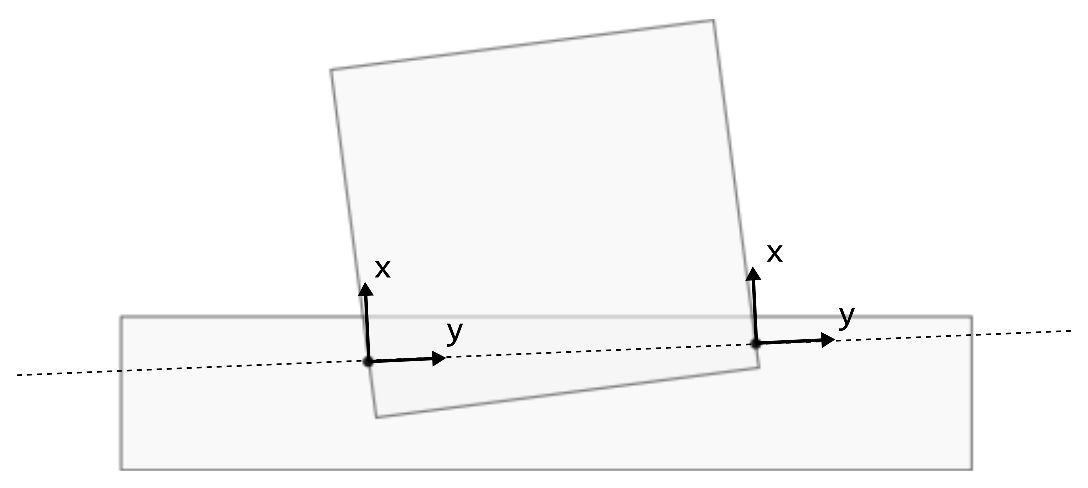
\includegraphics[clip, width=.7\hsize]{fig/phcontact.eps} \\
\end{tabular}
\end{center}
\caption{Contact configuration}
\label{fig_physics_contact}
\end{figure}

Springheadで採用している接触モデルについて説明します.
\KLUDGE 第\ref{sec_physics_scene}節で述べたように,\texttt{PHSceneIf::Step}によってシミュレーションを1ステップ進めると,
\KLUDGE 初めに形状の交差判定と接触拘束の生成が行われます.
\KLUDGE 交差する二つの形状の交差断面と,接触拘束の関係についてFig.\,\ref{fig_physics_contact}に示します.
\KLUDGE 図では簡単のために二次元で描いていますが,実際には接触断面を表す多角形の各頂点に接触拘束が作られます.
\KLUDGE 接触拘束も他の拘束と同様にソケットとプラグで構成されます.
\KLUDGE 一方で,他の拘束とは違い接触拘束は交差判定アルゴリズムによって動的に生成・破棄されます.
\KLUDGE このため,接触し合う剛体のどちらにソケットあるいはプラグが取り付けられるかは状況依存であり,外部から選択することはできません.

\KLUDGE プラグおよびソケットの向きは次のようにして決まります.
\KLUDGE まず,x軸は接触法線と平行に向きます.ただしどちらが正の向きかは状況依存です.
\KLUDGE 次に,y軸は接触点における二つの剛体の相対速度ベクトルを接触断面へ投影した向きに向きます.
\KLUDGE 最後にz軸はx,y軸に直交するように決まります.

\KLUDGE 以下では各接触拘束が課す条件について具体的に述べます.
\KLUDGE まず,法線方向の進入速度の大小に応じて衝突モデルと静的接触モデルのいずれかが選択されます.
\begin{align*}
v^\mathrm{x} < -V^\mathrm{th}   \;\; &\Rightarrow \;\; \text{衝突モデル} \\
v^\mathrm{x} \ge -V^\mathrm{th} \;\; &\Rightarrow \;\; \text{静的接触モデル}
\end{align*}
\KLUDGE ここで$v^\mathrm{x}$はソケットから見たプラグの相対速度のx軸(接触法線)成分で,近づき合う向きを負とします.
\KLUDGE また,$V^\mathrm{th}$は衝突モデルへ切り替わる臨界速度です.

\KLUDGE 衝突モデルでは,1ステップ後の相対速度${v^\mathrm{x}}'$が跳ね返り係数$e$にもとづいて決まり,それを満たすような接触力が計算されます.
\begin{align}
{v^\mathrm{x}}' = - e \, v^\mathrm{x}
\end{align}
\KLUDGE ここで,跳ね返り係数は衝突する形状の物性値に定義された跳ね返り係数の平均値です.
\KLUDGE %各形状の跳ね返り係数は,\texttt{CDShapeDesc::e}か,\texttt{CDShapeIf::SetElasticity}を用いて設定します
\KLUDGE %(第\ref{sec_collision_material}節参照).

\KLUDGE 静的接触モデルでは,形状同士の進入深度$d$が1ステップで所定の割合で減少するような接触力を求めます.
\KLUDGE つまり,1ステップ後の進入深度を$d'$とすると
\begin{align}
d' = d - \gamma \mathrm{max}(d - d^\mathrm{tol}, 0)
\end{align}
\KLUDGE となります.
\KLUDGE ここで$\gamma$は接触拘束の誤差修正率です.
\KLUDGE また,$d^\mathrm{tol}$は許容進入深度です.

\KLUDGE 最後に,接触力が満たすべき条件について述べます.
\KLUDGE まず,法線方向には反発力のみ作用することから,接触力のx軸成分$f^\mathrm{x}$には
\begin{align*}
f^\mathrm{x} \ge 0
\end{align*}
\KLUDGE が課せられます.
\KLUDGE 一方で接触力のy軸成分$f^\mathrm{y}$,z軸成分$f^\mathrm{z}$は摩擦力を表します.
\KLUDGE 摩擦力に関しては,その向きの相対速度にもとづき静止摩擦か動摩擦かが判定され,それに応じて最大摩擦力の制約が課されます.
\begin{align*}
\KLUDGE -\mu_0 f^\mathrm{x} \le &f^\mathrm{y} \le \mu_0 f^\mathrm{x} & & \text{if} \; -V^\mathrm{f} \le v^\mathrm{y} \le V^\mathrm{f},\\
 \mu   f^\mathrm{x} \le &f^\mathrm{y} \le \mu   f^\mathrm{x} & & \text{otherwise}
\end{align*}
\KLUDGE ここで,静止摩擦係数$\mu_0$および動摩擦係数$\mu$は跳ね返り係数と同様に各形状の物性値の平均値が用いられます.
\KLUDGE また,$V^\mathrm{f}$は静止摩擦と動摩擦が切り替わる臨界速度です.
z軸方向についても同様の制約が課されます.

\KLUDGE 接触モデルの関係するインタフェースには以下があります.
\begin{center}
\begin{longtable}{p{.1\hsize}p{.5\hsize}p{.4\hsize}}
\multicolumn{3}{l}{\texttt{CDShapeIf}}						\\ \midrule
\texttt{void}	& \texttt{SetElasticity(float e)}       & 跳ね返り係数を設定 \\
\texttt{float}  & \texttt{GetElasticity()}              & 跳ね返り係数を取得 \\
\texttt{void}   & \texttt{SetStaticFriction(float mu0)} & 静摩擦係数を設定 \\
\texttt{float}  & \texttt{GetStaticFriction()}          & 静摩擦係数を取得 \\
\texttt{void}   & \texttt{SetDynamicFriction(float mu)} & 動摩擦係数を設定 \\
\texttt{float}  & \texttt{GetDynamicFriction()}         & 動摩擦係数を取得
\end{longtable}
\end{center}

\begin{center}
\begin{longtable}{p{.1\hsize}p{.5\hsize}p{.4\hsize}}
\multicolumn{3}{l}{\texttt{PHSceneIf}}						\\ \midrule
\texttt{void}	& \texttt{SetContactTolerance(double tol)} & 許容交差深度を設定 \\
\texttt{double} & \texttt{GetContactTolerance()}           & 許容交差深度を取得 \\
\texttt{void}   & \texttt{SetImpactThreshold(double vth)}  & 最小衝突速度を設定 \\
\texttt{double} & \texttt{GetImpactThreshold()}            & 最小衝突速度を取得 \\
\texttt{void}   & \texttt{SetFrictionThreshold(double vf)} & 最小動摩擦速度を設定 \\
\texttt{double} & \texttt{GetFrictionThreshold()}          & 最小動摩擦速度を取得
\end{longtable}
\end{center}

\noindent\textbf{備考}
\begin{itemize}
\item 接触断面の向きについては,形状同士の進入速度をもとに決定しますが,ここでは詳しく述べません.
\item 摩擦力に関してはy軸,z軸が個別に扱われますが,実際の摩擦力はy成分とz成分の合力として与えられますので,
\KLUDGE 合力が最大摩擦力を超過する可能性があります.このようにSpringheadの摩擦モデルはあくまで近似的なものですので
\KLUDGE 注意して下さい.
\end{itemize}

\subsection*{接触力の取得}

\KLUDGE 特定の剛体に作用する接触力を直接取得するためのインタフェースは用意されていません.
\KLUDGE このため,ユーザサイドである程度の計算を行う必要があります.
\KLUDGE 以下に,ある剛体に作用する接触力の合力を求める例を示します.

\begin{sourcecode}
// given PHSceneIf* scene
// given PHSolidIf* solid

Vec3d fsum;    //< sum of contact forces applied to "solid"
Vec3d tsum;    //< sum of contact torques applied to "solid"

int N = scene->NContacts();
Vec3d f, t;
Posed pose;

for(int i = 0; i < N; i++){
    PHContactPointIf* con = scene->GetContact(i);
    con->GetConstraintForce(f, t);

    if(con->GetSocketSolid() == solid){
        con->GetSocketPose(pose);
        fsum -= pose.Ori() * f;
        tsum -= pose.Pos() % pose.Ori() * f;
    }
    if(con->GetPlugSolid() == solid){
        con->GetPlugPose(pose);
        fsum += pose.Ori() * f;
        tsum += pose.Pos() % pose.Ori() * f;
    }
}
\end{sourcecode}
\KLUDGE まず,シーン中の接触拘束の数を\texttt{PHSceneIf::NConstacts}で取得し,
\texttt{for}ループ中で$i$番目の接触拘束を\texttt{PHSceneIf::GetContact}で取得します.
\KLUDGE 次に\texttt{PHConstraintIf::GetConstraintForce}で接触力の並進力\texttt{f}とモーメント\texttt{t}を取得しますが,
\KLUDGE 接触拘束の場合モーメントは$0$ですので用いません.
\KLUDGE また,得られる拘束力はソケット/プラグ座標系で表したもので,作用点はソケット/プラグ座標系の原点です.
\KLUDGE これを考慮して剛体に作用する力とモーメントへ変換し,合力に足し合わせていきます.
\KLUDGE 剛体がソケット側である場合は作用・反作用を考慮して符号を反転することに注意して下さい.


\subsection*{接触力計算の有効/無効の切り替え}

\KLUDGE 多くのアプリケーションでは,すべての剛体の組み合わせに関して接触を取り扱う必要はありません.
\KLUDGE このような場合は必要な剛体の対に関してのみ接触を有効化することで計算コストを削減できます.
Springheadでは,剛体の組み合わせ毎に交差判定および接触力計算を行うかを切り替えることができます.
\KLUDGE これには\texttt{PHSceneIf::SetContactMode}を用います.

\begin{center}
\begin{longtable}{p{.1\hsize}p{.9\hsize}}
\multicolumn{2}{l}{\texttt{PHSceneIf}}						\\ \midrule
\texttt{void}	& \texttt{SetContactMode(PHSolidIf* lhs, PHSolidIf* rhs, int mode)} \\
\texttt{void}   & \texttt{SetContactMode(PHSolidIf** group, size\_t length, int mode)} \\
\texttt{void}   & \texttt{SetContactMode(PHSolidIf* solid, int mode)} \\
\texttt{void}   & \texttt{SetContactMode(int mode)}
\end{longtable}
\end{center}

\KLUDGE 一番目は剛体\texttt{lhs}と\texttt{rhs}の対に関してモードを設定します.
\KLUDGE 二番目は配列\texttt{[group, group + length]}に格納された剛体の全組み合わせに関して設定します.
\KLUDGE 三番目は剛体\texttt{solid}と他の全剛体との組み合わせに関して設定します.
\KLUDGE 四番目はシーン中のすべての剛体の組み合わせに関して設定します.

\KLUDGE 設定可能なモードは以下の内の一つです.
\begin{center}
\begin{longtable}{p{.3\hsize}p{.7\hsize}}
\multicolumn{2}{l}{\texttt{PHSceneDesc::ContactMode}} \\ \midrule
\texttt{MODE\_NONE}	   & 交差判定および接触力計算を行わない \\
\texttt{MODE\_LCP}     & 交差判定を行い,拘束力計算法を用いる \\
\texttt{MODE\_PENALTY} & 交差判定を行い,ペナルティ反力法を用いる \\
\end{longtable}
\end{center}
\KLUDGE デフォルトではすべての剛体対に関して\texttt{MODE\_LCP}が選択されています.
\KLUDGE 例として,床面との接触以外をすべてオフにするには
\begin{sourcecode}
// given PHSolidIf* floor

scene->SetContactMode(PHSceneDesc::MODE_NONE);
scene->SetContactMode(floor, PHSceneDesc::MODE_LCP);
\end{sourcecode}
\KLUDGE とします.

\section{関節座標系シミュレーション}

\index{かんせつざひょうけい@関節座標系}
T.B.D.


\section{ギア}

\index{ぎあ@ギア}
T.B.D.

\section{内部アルゴリズムの設定}
\label{sec_physics_engine}

\KLUDGE 以下では物理シミュレーションの内部で用いられているアルゴリズムの詳細な設定項目について説明します.

\subsection*{拘束力計算エンジン}

\KLUDGE 拘束力計算エンジンは,関節や接触などの拘束を満足するための拘束力の計算を行います.
\KLUDGE 拘束力計算エンジンのクラスは\texttt{PHConstraintEngineIf}で,これを取得するには以下の関数を用います.


\texttt{PHConstraintEngineIf}のインタフェースを以下に示します.

\begin{center}
\begin{longtable}{p{.12\hsize}p{.45\hsize}p{.33\hsize}}
\multicolumn{3}{l}{\texttt{PHConstraintEngineIf}}			\\ \midrule
\texttt{void}	& \texttt{SetVelCorrectionRate(double)}		& 関節拘束の誤差修正率を設定 \\
\texttt{double} & \texttt{GetVelCorrectionRate()}			& 関節拘束の誤差修正率を取得 \\
\texttt{void}	& \texttt{SetContactCorrectionRate(double)}	& 接触拘束の誤差修正率を設定 \\
\texttt{double} & \texttt{GetContactCorrectionRate()}		& 接触拘束の誤差修正率を取得 \\
\end{longtable}
\end{center}

\KLUDGE 誤差修正率とは,1ステップで拘束誤差どの程度修正するかを示す比率で,通常$[0, 1]$の値を設定します.
\KLUDGE 誤差修正率を$1$にすると,1ステップで拘束誤差を$0$にするような拘束力が計算されますが,発振現象などのシミュレーションの不安定化を招く傾向があります.
\KLUDGE 逆に修正率を小さ目に設定すればシミュレーションは安定化しますが,定常誤差が増大します.

\KLUDGE 拘束力計算エンジンは,内部で反復型のアルゴリズムで拘束力を計算します.
\KLUDGE アルゴリズムの反復回数は\texttt{PHSceneIf::SetNumIteration}で設定します(第\ref{sec_physics_scene}節参照).


\texttt{PHSceneIf::SetContactTolerance}で設定可能です.

\texttt{PHConstraintEngineIf::SetContactCorrectionRate}で設定可能です
\KLUDGE (第\ref{sec_physics_engine}節参照).
